\subsection{TADIP}
\label{sec:algorithms:tadip}

\begin{figure}[H]
    \centering
    \begin{subfigure}[b]{0.45\textwidth}
        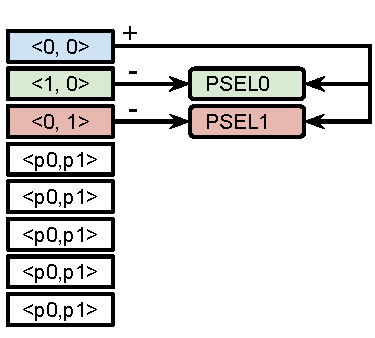
\includegraphics[width=\textwidth]{figures/algorithms/TADIP-I}
        \caption{Cache managed by \gls{tadip-i}.}
        \label{fig:algorithms:tadip:isolated}
    \end{subfigure}
    \begin{subfigure}[b]{0.45\textwidth}
        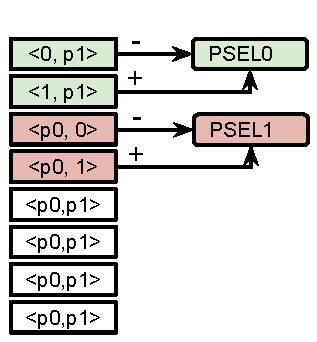
\includegraphics[width=\textwidth]{figures/algorithms/TADIP-F}
        \caption{Cache managed by \gls{tadip-f}.}
        \label{fig:algorithms:tadip:feedback}
    \end{subfigure}    
    \caption{Alternate duel set organizations for \gls{tadip}.}
    \label{fig:algorithms:tadip}
\end{figure}

\gls{tadip}~\cite{Jaleel2008} proposed in 2008 is a thread-aware extension of \gls{dip}~\cite{Qureshi2007}.
The main issue with \gls{dip} that \gls{tadip} counters, is that \gls{dip} does not consider which core initiates a cache access.
In a workload with multiple benchmarks, some might be recency-friendly while others are not. 
In a shared cache managed by \gls{dip}, the algorithm choice is made based on the sum of the cache accesses and then applied equally to all cores.
The authors of \gls{tadip} recognized that improvements in performance could be achieved by selecting the \gls{dip} policy on a per-core basis when utilized in a shared cache.

When selecting the best performing algorithm per core, the \gls{atd} technique requires two \glspl{atd} per core sharing the cache. 
This solution can quickly become too expensive to be practical.
Set-dueling in \gls{dip} requires a minimum of two sets, one running \gls{lip} (1) and one running \gls{bip} (0). 
With two cores, the number of combinations rises to four (00, 01, 10, 11).
When the number of cores increases this also seems to be an impractical solution.
Based on this observation, the authors of \gls{tadip} suggested two new selection techniques based on set dueling, which reduce the number of duel sets required.
Both solutions have one saturating counter per core sharing the cache.
This counter is used to select the best performing policy for that core.

\gls{tadip-i} has one set per core running \gls{bip} for that core and \gls{lip} for all others.
In addition to these N sets, a single set runs \gls{lip} for all cores. 
A miss in the \gls{lip} set will increment all the core counters while a miss in the core specific set will decrement the counter for the specific core.
For a large N, this solution requires significantly fewer duel sets compared to having one per combination ($N+1 << N^2$). 
This solution assumes that all other cores run \gls{lip}, and, therefore, cannot fully capture the effect of interactions between cores.
Figure~\ref{fig:algorithms:tadip:isolated} shows an example of a cache managed by \gls{tadip-i}. 
In the figure, PSEL0 is the saturating counter used to select the best performing policy for core 0.
Within a set; $<0, 0>$ indicates that both cores run \gls{lip} while $<1, 0>$ indicates that core 0 runs \gls{bip} while core 1 runs \gls{lip}.
The variables p0 and p1 represent the current best performing policy for core 0 and 1 respectively.

\gls{tadip-f} attempts to reduce the error caused by the assumption of other cores by having two sets per core, a total of 2N.
A cache managed by \gls{tadip-f} is illustrated in Figure~\ref{fig:algorithms:tadip:feedback}.
For each of the cores, one duel set use \gls{lip} and the other use \gls{bip}. 
Any insertions from other cores into the duel sets use the current best performing algorithm for that core.
Like in the other policies, a miss in the \gls{lip} set for a core will increment that core's counter and a miss the \gls{bip} set will decrement the counter.
For the remainder of this thesis when we refer to \gls{tadip} we assume \gls{tadip-f} unless otherwise stated.

When implementing \gls{tadip}, some mechanism is required to select which sets are duel sets, and which are follower sets.
The authors of \gls{tadip} provide a simple hash function that can be used to select dueling sets, shown in Algorithm~\ref{alg:algorithms:tadip:set_selection}.
This algorithm assumes a 4096 set cache.
In the algorithm, set index is a number from 0-4095, core\_id is the zero-indexed id of the requester core and cores is the total number of cores sharing the cache.
If \gls{bip} or \gls{lip} is true, then the set is a duel set for the given core, and the policy forced to either \gls{bip} or \gls{lip}.
If both \gls{bip} and \gls{lip} are false, then the set is a normal follower set and utilizes the current best performing algorithm for the given core.
It follows from the algorithms that the original authors use a total of 32 duel sets spread evenly throughout the cache.

\begin{algorithm}[ht]
\caption{TADIP duel set selection.}
\label{alg:algorithms:tadip:set_selection}
\begin{algorithmic}[1]
\State $LIP\gets set\_no[11:7] + core\_id == set\_no[6:0]$
\State $BIP\gets set\_no[11:7] + core\_id + cores == set\_no[6:0]$
\State $FOLLOWER\gets !LIP + !BIP$
\end{algorithmic}
\end{algorithm}
